% ****************************************************************************************
% *********************        SISTEMAS OPERATIVOS            ****************************
% ****************************************************************************************

% =======================================================
% =======         HEADER FOR DOCUMENT        ============
% =======================================================
    % *********   DOCUMENT ITSELF   **************
    \documentclass[12pt, fleqn]{report}                             %Type of docuemtn and size of font and left eq
    \usepackage[margin=1.2in]{geometry}                             %Margins and Geometry pacakge
    \usepackage{ifthen}                                             %Allow simple programming
    \usepackage{hyperref}                                           %Create MetaData for a PDF and LINKS!
    \setlength{\parindent}{0pt}                                     %Eliminate ugly indentation
    \author{Oscar Andrés Rosas}                                     %Who I am

    % *********   LANGUAJE AND UFT-8   *********
    \usepackage[spanish]{babel}                                     %Please use spanish
    \usepackage[utf8]{inputenc}                                     %Please use spanish - UFT
    \usepackage[T1]{fontenc}                                        %Please use spanish
    \usepackage{textcmds}                                           %Allow us to use quoutes
    \usepackage{changepage}                                         %Allow us to use identate paragraphs

    % *********   MATH AND HIS STYLE  *********
    \usepackage{ntheorem, amsmath, amssymb, amsfonts}               %All fucking math, I want all!
    \usepackage{mathrsfs, mathtools, empheq}                        %All fucking math, I want all!
    \usepackage{centernot}                                          %Allow me to negate a symbol
    \decimalpoint                                                   %Use decimal point

    % *********   GRAPHICS AND IMAGES *********
    \usepackage{graphicx}                                           %Allow to create graphics
    \usepackage{wrapfig}                                            %Allow to create images
    \usepackage{xcolor}                                             %Allow to create images
    \graphicspath{ {Graphics/} }                                    %Where are the images :D

    % *********   LISTS AND TABLES ***********
    \usepackage{listings}                                           %We will be using code here
    \usepackage[inline]{enumitem}                                   %We will need to enumarate
    \usepackage{tasks}                                              %Horizontal lists
    \usepackage{longtable}                                          %Lets make tables awesome
    \usepackage{booktabs}                                           %Lets make tables awesome
    \usepackage{tabularx}                                           %Lets make tables awesome
    \usepackage{multirow}                                           %Lets make tables awesome
    \usepackage{multicol}                                           %Create multicolumns

    % *********   HEADERS AND FOOTERS ********
    \usepackage{fancyhdr}                                           %Lets make awesome headers/footers
    \pagestyle{fancy}                                               %Lets make awesome headers/footers
    \setlength{\headheight}{16pt}                                   %Top line
    \setlength{\parskip}{0.5em}                                     %Top line
    \renewcommand{\footrulewidth}{0.5pt}                            %Bottom line

    \lhead{                                                         %Left Header
        \hyperlink{chapter.\arabic{chapter}}                        %Make a link to the current chapter
        {\normalsize{\textsc{\nouppercase{\leftmark}}}}             %And fot it put the name
    }

    \rhead{                                                         %Right Header
        \hyperlink{section.\arabic{chapter}.\arabic{section}}       %Make a link to the current chapter
            {\footnotesize{\textsc{\nouppercase{\rightmark}}}}      %And fot it put the name
    }

    \rfoot{\textsc{\small{\hyperref[sec:Index]{Ve al Índice}}}}     %This will always be a footer  

    \fancyfoot[L]{                                                  %Algoritm for a changing footer
        \ifthenelse{\isodd{\value{page}}}                           %IF ODD PAGE:
            {\href{https://compilandoconocimiento.com/yo/}          %DO THIS:
                {\footnotesize                                      %Send the page
                    {\textsc{Oscar Andrés Rosas}}}}                 %Send the page
            {\href{https://compilandoconocimiento.com}              %ELSE DO THIS: 
                {\footnotesize                                      %Send the author
                    {\textsc{Compilando Conocimiento}}}}            %Send the author
    }
    
    
    
% ========================================
% ===========   COMMANDS    ==============
% ========================================

    % =====  GENERAL TEXT  ==========
    \newcommand \Quote {\qq}                                        %Use: \Quote to use quotes
    \newcommand \Over {\overline}                                   %Use: \Bar to use just for short
    \newcommand \ForceNewLine {$\Space$\\}                          %Use it in theorems for example
    
    \newenvironment{Indentation}[1][0.75em]                         %Use: \begin{Inde...}[Num]...\end{Inde...}
    {\begin{adjustwidth}{#1}{}}                                     %If you dont put nothing i will use 0.75 em
    {\end{adjustwidth}}                                             %This indentate a paragraph
    \newenvironment{SmallIndentation}[1][0.75em]                    %Use: The same that we upper one, just 
    {\begin{adjustwidth}{#1}{}\begin{footnotesize}}                 %footnotesize size of letter by default
    {\end{footnotesize}\end{adjustwidth}}                           %that's it


    % =====  GENERAL COLOR  =========
    \definecolor{IndigoMD}{HTML}{3F51B5}                            %Use: Color :D
    \definecolor{DeepPurpleMD}{HTML}{673AB7}                        %Use: Color :D
    \definecolor{TealMD}{HTML}{009688}                              %Use: Color :D

    \newenvironment{ColorText}[1]{                                  %Use: \begin{ColorText}
        \leavevmode\color{#1}\ignorespaces}                         %That's is!

            
    % =====  GENERAL MATH  ==========
    \DeclareMathOperator \Space {\quad}                             %Use: \Space for a cool mega space
    \DeclareMathOperator \MiniSpace {\;}                            %Use: \Space for a cool mini space
    \newcommand \Such {\MiniSpace|\MiniSpace}                       %Use: \Such like in sets
    \newcommand \Also {\Space \text{y} \Space}                      %Use: \Also so it's look cool
    \newcommand \Remember[1]{\Space\text{\scriptsize{#1}}}          %Use: \Remember so it's look cool

    \newtheorem{Theorem}{Teorema}[section]                          %Use: \begin{Theorem}[Name]\label{Nombre}...
    \newtheorem{Corollary}{Colorario}[Theorem]                      %Use: \begin{Corollary}[Name]\label{Nombre}...
    \newtheorem{Lemma}[Theorem]{Lemma}                              %Use: \begin{Lemma}[Name]\label{Nombre}...
    \newtheorem{Definition}{Definición}[section]                    %Use: \begin{Definition}[Name]\label{Nombre}...

    \newcommand{\Set}[1]{\left\{ \MiniSpace #1 \MiniSpace \right\}} %Use: \Set {Info}
    \newcommand{\Brackets}[1]{\left[ #1 \right]}                    %Use: \Brackets {Info} 
    \newcommand{\Wrap}[1]{\left( #1 \right)}                        %Use: \Wrap {Info} 
    \newcommand{\pfrac}[2]{\Wrap{\dfrac{#1}{#2}}}                   %Use: Put fractions in parentesis

    \newenvironment{MultiLineEquation}[1]                           %Use: To create MultiLine equations
        {\begin{equation}\begin{alignedat}{#1}}                     %Use: \begin{Multi..}{Num. de Columnas}
        {\end{alignedat}\end{equation}}                             %And.. that's it!
    \newenvironment{MultiLineEquation*}[1]                          %Use: To create MultiLine equations
        {\begin{equation*}\begin{alignedat}{#1}}                    %Use: \begin{Multi..}{Num. de Columnas}
        {\end{alignedat}\end{equation*}}                            %And.. that's it!


    % =====  LOGIC  ==================
    \DeclareMathOperator \doublearrow {\leftrightarrow}             %Use: \doublearrow for a double arrow
    \newcommand \lequal {\MiniSpace \Leftrightarrow \MiniSpace}     %Use: \lequal for a double arrow
    \newcommand \linfire {\MiniSpace \Rightarrow \MiniSpace}        %Use: \lequal for a double arrow
    \newcommand \longto {\longrightarrow}                           %Use: \longto for a long arrow

    % =====  NUMBER THEORY  ==========
    \DeclareMathOperator \Naturals  {\mathbb{N}}                     %Use: \Naturals por Notation
    \DeclareMathOperator \Primes    {\mathbb{P}}                     %Use: \Naturals por Notation
    \DeclareMathOperator \Integers  {\mathbb{Z}}                     %Use: \Integers por Notation
    \DeclareMathOperator \Racionals {\mathbb{Q}}                     %Use: \Racionals por Notation
    \DeclareMathOperator \Reals     {\mathbb{R}}                     %Use: \Reals por Notation
    \DeclareMathOperator \Complexs  {\mathbb{C}}                     %Use: \Complex por Notation

    % === LINEAL ALGEBRA & VECTORS ===
    \DeclareMathOperator \LinealTransformation {\mathcal{T}}        %Use: \LinealTransformation for a cool T

    \newcommand{\pVector}[1]{                                       %Use: \pVector {Matrix Notation} use parentesis
        \ensuremath{\begin{pmatrix}#1\end{pmatrix}}                 %Example: \pVector{a\\b\\c} or \pVector{a&b&c} 
    }
    \newcommand{\lVector}[1]{                                       %Use: \lVector {Matrix Notation} use a abs 
        \ensuremath{\begin{vmatrix}#1\end{vmatrix}}                 %Example: \lVector{a\\b\\c} or \lVector{a&b&c} 
    }
    \newcommand{\bVector}[1]{                                       %Use: \bVector {Matrix Notation} use a brackets 
        \ensuremath{\begin{bmatrix}#1\end{bmatrix}}                 %Example: \bVector{a\\b\\c} or \bVector{a&b&c} 
    }
    \newcommand{\Vector}[1]{                                        %Use: \Vector {Matrix Notation} no parentesis
        \ensuremath{\begin{matrix}#1\end{matrix}}                   %Example: \Vector{a\\b\\c} or \Vector{a&b&c}
    }
    \newcommand{\uvec}[1]{\boldsymbol{\hat{\textbf{$#1$}}}}         %Use: Unitary Vector

    % MATRIX
    \makeatletter                                                   %Example: \begin{matrix}[cc|c]
    \renewcommand*\env@matrix[1][*\c@MaxMatrixCols c] {             %WTF! IS THIS
        \hskip -\arraycolsep                                        %WTF! IS THIS
        \let\@ifnextchar\new@ifnextchar                             %WTF! IS THIS
        \array{#1}                                                  %WTF! IS THIS
    }                                                               %WTF! IS THIS
    \makeatother                                                    %WTF! IS THIS

    % TRIGONOMETRIC FUNCTIONS
    \newcommand{\Cos}[1]{\cos\Wrap{#1}}
    \newcommand{\Sin}[1]{\sin\Wrap{#1}}

    % === CALCULUS ===                               
    \newcommand \Derivate[2] {\dfrac{d #1}{d#2}}                    %Use: Derivate Notation
    \newcommand \Partial[2] {\dfrac{\partial #1}{\partial#2}}       %Use: Derivate Partial Notation
    
    \newcommand \pDerivate[2]{\Derivate{\Wrap{#1}}{#2}}             %But with cool parentesis
    \newcommand \pPartial[2]{\Partial{\Wrap{#1}}{#2}}               %Use: Derivate Partial
    
    \newcommand \SemiDerivate[1]{\Wrap{\dfrac{d}{d#1}}}             %Use: Derivate Notation
    \newcommand \SemiPartial[1]{\Wrap{\dfrac{\partial}{\partial#1}}}%Use: Derivate Partial Notation


    % === COMPLEX ANALYSIS ===
    \newcommand \Cis[1]  {\Cos{#1} + i \Sin{#1}}                    %Use: \Cis for cos(x) + i sin(x)
    \newcommand \pCis[1] {\Wrap{\Cis{#1}}}                          %Use: \pCis for the same ut parantesis










% =====================================================
% ============        COVER PAGE       ================
% =====================================================
\begin{document}
\begin{titlepage}

    \center
    % ============ UNIVERSITY NAME AND DATA =========
    \textbf{\textsc{\Large Proyecto Compilando Conocimiento}}\\[1.0cm] 
    \textsc{\Large Programación}\\[1.0cm] 

    % ============ NAME OF THE DOCUMENT  ============
    \rule{\linewidth}{0.5mm} \\[1.0cm]
        { \huge \bfseries Bases de Sistemas Operativos}\\[1.0cm] 
    \rule{\linewidth}{0.5mm} \\[2.0cm]
    
    % ====== SEMI TITLE ==========
    {\LARGE Una Pequeña (Gran) Introducción}\\[7cm] 
    
    % ============  MY INFORMATION  =================
    \begin{center} \large
    \textbf{\textsc{Autores:}}\\
        Rosas Hernandez Oscar Andrés \\
        Lopez Manriquez Angel
    \end{center}

    \vfill

\end{titlepage}

% =====================================================
% ========                INDICE              =========
% =====================================================
\tableofcontents{}
\label{sec:Index}

\clearpage




% //////////////////////////////////////////////////////////////////////////////////////////////////////////
% ///////////////////////////////////              INTRODUCCION            /////////////////////////////////
% //////////////////////////////////////////////////////////////////////////////////////////////////////////
\part{Una Introducción}
\clearpage


    % ===============================================================================
    % ===================           DEFINICIONES               ======================
    % ===============================================================================
    \chapter{Introducción}

        % ==============================================
        % ========    REPOSITORIO DE DATOS     =========
        % ==============================================
        \clearpage
        \section{¿Qué es un Sistema Operativo?}
            
            Los sistemas operativos surgen como una solución a la problematica de la 
            \textbf{ administración de un equipo de computo}, de forma tal que fuese más sencillo
            trabajar con el y aprovechar al máximo sus recursos.
    
            "Un sistema operativo es un programa encargado de controlar todos lor recursos de
            una copmutadora"

            \subsection{Definición Formal}

                \Quote{Un sistema operativo es un software de base compuesto por un conjunto
                de administradores encargados de la administracion de cada uno de los recursos
                de un equipo de coputo de forma rápida y eficiente.}


                \subsection*{Características}

                    \begin{itemize}
                        \item 
                            Un sistema operativo es un software de base debido a que es una plataforma que permite
                            la creación y ejecución de aplicaciones desarrolladas para el propio sistema.
                            Como software de base, el sistem operativo ofrece interfaces para la creación o ejecución
                            de las aplicaciones desarrolladas.

                        \item
                            Un sistema operativo esta compuesto de un conjunto de administradores, los cuales controlan
                            todos los recursos del equipo de computo, estos administradores son: 

                            \begin{itemize}
                                \item Administrador de Procesos
                                \item Admin. de Memoria 
                                \item Admin. de Entrada / Salida 
                                \item Admin. de Archivos 
                                \item Admin. de Red 
                            \end{itemize}

                        \item
                            Un sistema operativo debe ejecutarse lo más rapido posible, evitando quitarle tiempo de
                            procesamiento a las aplicaciones de los usuarios, por otro lado debe administrar cada uno
                            de los recursos del equipo de cómputo de forma eficiente, maximizando el uso de cada
                            recurso controlado. 
                            La rápidez y eficiencia es uno de los principales u objetivos que un Sistema Operativo debe
                            cumplir durante su ejecución.
                
                    \end{itemize}
       

        % ==============================================
        % ========    TIPO DE SISTEMAS         =========
        % ==============================================
        \section{Tipo de Sistemas}

            Sistemas Genericos:
            \begin{itemize}
                \item Por lotes sencillos
                \item Por lotes multiprogramados
                \item De tiempo compartido
            \end{itemize}

            Sistemas Distribuidos:
            \begin{itemize}
                \item Distribuidos: En estos los procesadores no comparten el mismo reloj ni memoria, son sistemas
                    debilmente acomplados
                \item Paralela: Los procesadores comparten los recursos como la memoria, son sistemas fuertemente
                    acomplados
            \end{itemize}     

        % ==============================================
        % ========      TERMINOS COMUNES       =========
        % ==============================================
        \clearpage
        \section{Terminos Básicos}

            \begin{itemize}
                \item
                    \textbf{Spooling: }

                    SPOOL significa \Quote{Simultaneous Peripheral Operation On-Line}.

                    En realidad, lo que sucede aquí es que hay buffer para almacenar los datos,
                    por lo general el disco.

                    Los dispositivos de entrada / salida no pueden trabajar a la velocidad de una CPU.
                    Por lo tanto, la salida de la CPU se almacenará en este spool (buffer) y los
                    dispositivos de entrada / salida pueden tomar la salida de este buffer como y cuando
                    se requiera de acuerdo a su velocidad.

                    Por lo tanto, la CPU no está vinculada a este dispositivo de entrada / salida y
                    puede realizar otras operaciones.
                    Gracias al spooling podemos mantener la CPU y los dispositivos de entrada y salida
                    trabajando a altas velocidades sin esperar el uno al otro.

                \item
                    \textbf{Reserva de Trabajo: }

                    Conjunto de trabajos en el disco listos para ser ejecutados por la CPU

                \item
                    \textbf{Planificación de Trabajo: }

                    Es la técnica que se encarga de seleccionar cual será el siguiente trabajo
                    ejecutado en la CPU.

                \item
                    \textbf{Multiprogramación: }

                    Técnica utilizada para almacenar múltiples trabajos simultáneamente en la 
                    memoria física (RAM).

                \item
                    \textbf{Tiempo Compartido: }

                    Técnica utilizada para asignar un tiempo de ejecución a cada proceso
                    lo suficientemente corto para conmutar entre ellos.

                    El sistema de tiempo compartido es donde cada proceso se asigna un período de
                    tiempo determinado y el proceso tiene que terminar su finalización dentro de ese
                    lapso de tiempo.

                    Si no se logra completar su ejecución, entonces el control de CPU pasa al
                    próximo proceso.

                \item
                    \textbf{Concurrencia: }

                    Técnica utilizada ejecutar múltiples trabajos bajo la apariencia de
                    simultaneidad o paralelismo mediante una ejecución secuencial.

                \item
                    \textbf{Memoria Virtual: }

                    Técnica utilizada para aumentar o extender la memoria física (RAM) mediante
                    el uso de una pequeña región de disco.

                \item
                    \textbf{Sistema de Archivos: }

                    Estructura de almacenamiento de información mediante entes llamados
                    archivos y directorios.

                \item
                    \textbf{Sistemas Paralelos: }

                    Sistemas utilizados para el multiprocesamiento compuesto por un conjunto
                    de procesadores que comparten el reljo, memoria y buses del equipo, por lo
                    que se conocen como fuertemente acoplados.

                \item
                    \textbf{Sistemas Distribuidos: }

                    istemas utilizados para el multiprocesamiento compuesto por un conjunto
                    de sistemas de cómputo completo que manejan de forma independiente cosas
                    como el reloj, la memoria o los buses. Por esto se le conoce como debilmente
                    acoplados.

            \end{itemize}



    % ===============================================================================
    % ===========          PARTES DEL SISTEMA OPERATIVO           ===================
    % ===============================================================================
    \chapter{Partes del Sistema Operativo}

        % ==============================================
        % =============    VISTA GENERAL    ============
        % ==============================================
        \clearpage
        \section{Vista General}

            Un Sistema Operativo como cualquier otro software sigue un modelo de ingeniería de
            software para su diseño y construcción, en modelo que se usa es el denominado por capas,
            este modelo nos dice que cada capa se encarga de realizar una funcionalidad concreta
            dentro del sistema operativo.

            Un sistema operativo normalmente está integrado por las siguientes capas:
            \begin{itemize}
                \item Hardware
                \item Kernel
                \item Servicios        
                \item Aplicaciones
            \end{itemize}  

            Estas capas para llevar a cabo sus funciones requieren comunicarse con cada adyacentes,
            para lograr esta comunicación se usan las interfaces,
            estas son:
            \begin{itemize}
                \item Interfaz de Comandos
                \item Interfaz de Llamafas al Sistema
                \item Interfaz de Interrupciones        
            \end{itemize}  


            Graficamente las podemos ver como:

            \begin{figure}[h!]
                \centering
                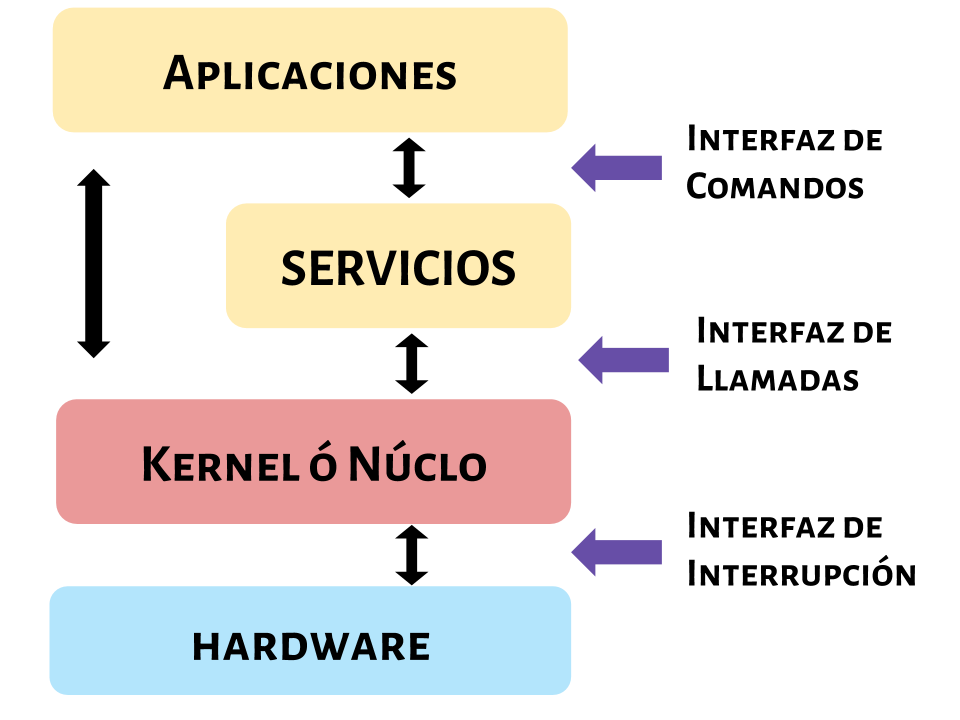
\includegraphics[width=0.55\textwidth]{Capas}
            \end{figure}

        % ==============================================
        % =============        CAPAS        ============
        % ==============================================
        \clearpage
        \section{Capas}    

            \begin{itemize}
                \item
                    \textbf{Capa de Aplicaciones}

                    Esta capa se encarga de mantener cualquier aplicación que el usuario ejecutará
                    en el sistema operativo, siendo la capa con la que el usuario tendrá contacto.

                    Se encarga de mantener todas las aplicaciones que tu conoces normalmente.


                \item
                    \textbf{Capa de Servicios}

                    Esta capa se encarga de mantener los servicio que apoyan el funcionamiento
                    del sistema operativo, teniendo servicios de seguridad, de mantenimiento,
                    entre otras.

                    A veces se suele unir y dividir sus funciones entre la capa de aplicaciones
                    y el kernel.


                \item
                    \textbf{Capa de Kernel o Núcleo}

                    Esta es la capa principal del sistema operativo, esta mantiene a los 5
                    administradores que componen a todo sistema operativo.


                \item
                    \textbf{Capa de Hardware}

                    Esta es la capa mas baja del sistema, se encarga de mantener todas las interfaces
                    de comunicación con el hardware.

            \end{itemize}


        % ==============================================
        % =========       INTERFACES        ============
        % ==============================================
        \clearpage
        \section{Interfaces}    
            
            \begin{itemize}
                \item
                    \textbf{Interfaz de Comandos}

                    Esta interfaz comunica a la capa de aplicaciones con la de
                    servicios o a la capa del kernel.

                    Esta compuesta de por todos los comandos disponibles en el sistema
                    operativo, siendo la interfaz de interacción inmediata que el usuario
                    posee para comunicarse con el sistema operativo.

                \item
                    \textbf{Interfaz de Llamadas al Sistema}

                    Esta interfaz comunica a la capa de servicios con la de
                    aplicaciones o a la capa del kernel.

                    Esta compuesta por unas APIs (es decir funciones o métodos)
                    que el sistema operativo pone a dispoción de los usuarios a
                    través de un lenguaje de alto nivel, por esto se le conoce como una
                    comunicación indirecta.

                \item
                    \textbf{Interfaz de Interrupciones}

                    Esta interfaz comunica a la capa del kernel con la del hardware.

                    Esta compuesta por un conjunto de interrupciones o servicios de 
                    interrupción que el sistema operativo pone a dispoción de los
                    usuarios por medio de un lenguaje de programación de bajo nivel,
                    por esto se le conoce como una comunicación indirecta.

            \end{itemize}





    % ===============================================================================
    % ===========         KERNEL DE UN SISTEMA OPERATIVO          ===================
    % ===============================================================================
    \chapter{Kernel de un Sistema Operativo}

        % ==============================================
        % ===========    ADMINISTRADORES    ============
        % ==============================================
        \clearpage
        \section{Conozcamos a los Administradores}

            Podemos separar el Kernel en varios administradores, todos interactuan entre si
            para realizar correctamente su trabajo.

            \begin{itemize}
                \item
                    \textbf{Administrador de Procesos:}

                    Se encarga de la ejecución de cualquier trabajo en el Sistema, esta
                    compuesto por un conjunto de algoritmos de planificación y de estructuras
                    de datos.

                    El hardware con el cual interactua este administrador es el procesador
                    del equipo de cómputo.

                \item
                    \textbf{Administrador de Memoria:}

                    Este administrador se encarga de la gestión tanto de la memoria física como
                    de la memoria virtual.

                    Esta compuesto por un esquema global de gestión de memoria, así como el
                    conjunto de algoritmos para el control de la memoria.


                \item
                    \textbf{Administrador de Entrada y Salida:}

                    Este administrador se encarga de la gestión de acceder a cualquier dispositivo
                    externo.
                    Esta compuesto por un conjunto de interfaces de conectividad y controladores
                    de nivel de hardware como software.


                \item
                    \textbf{Administrador de Archivos:}

                    Este administrador se encarga de la gestión de todos los archivos del
                    sistema operativo.
                    Se encarga de la organización lógica de la información.

                 \item
                    \textbf{Administrador de Red:}

                    Este administrador se encarga de cualquier comunicación en red del sistema
                    operativo, esta compuesto por un modelo de comunicación en red y diversos
                    protocolos asociados al modelo usado.

            \end{itemize}


            \begin{figure}[h!]
                \centering
                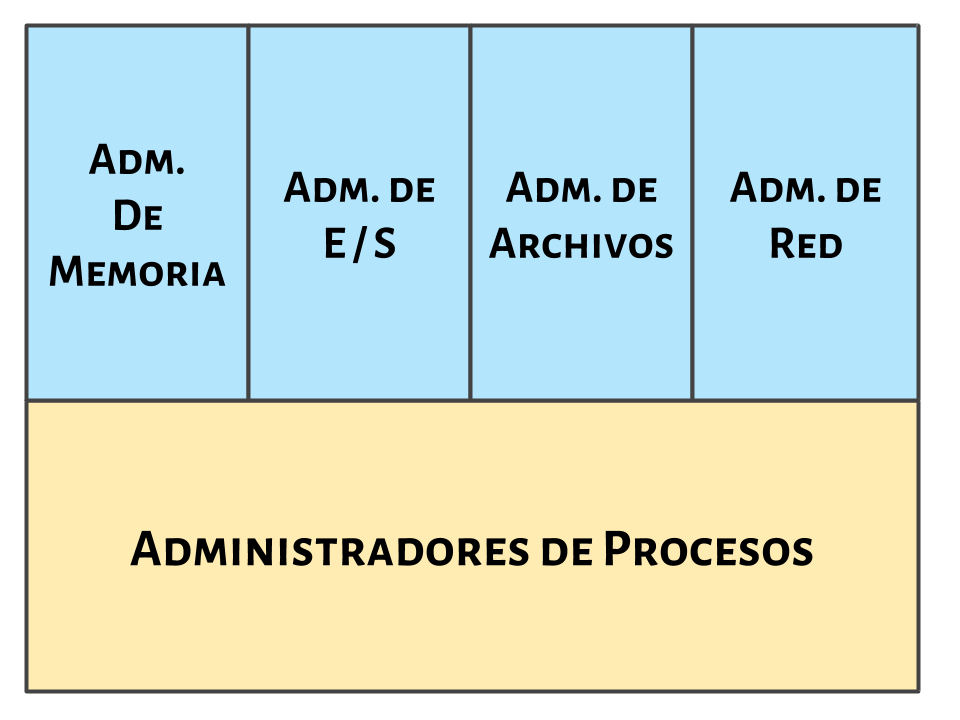
\includegraphics[width=0.85\textwidth]{PartesDelKernel}
            \end{figure}


    % ===============================================================================
    % ===========               ADMINISTRADOR DE PROCESOS         ===================
    % ===============================================================================
    \chapter{Administrador de Procesos}

        % ==============================================
        % ===========    ADMINISTRADORES    ============
        % ==============================================
        \clearpage
        \section{Introducción}

            Es uno de los principales administradores del sistema operativo.
            Este se encarga de la gestión de cualquier trabajo a ejecutar en el sistema.
            Los trabajos que son ejecutados por este administrador son llamados \textbf{procesos}.
            Se encarga de llevar a cabo la ejecución de todos los programas del sistema operativo.

            \subsection{Procesos}

                \begin{ColorText}{IndigoMD}
                    {\Quote{Un proceso es un programa en ejecución}}

                    \Quote{Un proceso es la entidad mínima de software ejecutándose en el Sistema
                    Operativo contenido en una estructura de infromación}

                \end{ColorText}

                De esta definición podemos obtener dos caracteristicas muy importantes:
                \begin{itemize}
                    
                    \item Es una Entidad de Software

                        \begin{SmallIndentation}
                            Esto implica que tendrá asociado un ciclo de vida. Este ciclo representará
                            las diverdad etapas por las cuales puede transitar un proceso.

                            Un proceso en el sistema operativo se implementará a través de una
                            estructura de información, la cual contendrá toda la información necesaria
                            para caracterizar a dicho proceso.

                            Esta estructura de información es implementada mediante una
                            estructura de datos en el lenguaje de alto nivel que estemos utilizando.

                            A esta estructura se le conoce como \textbf{Bloque de Control del Proceso}
                            (PCB). 

                            Este PCB es el elemento con el que el Administrador de Procesos
                            interacturá durante el ciclo de vida del proceso presente en el sistema 
                            operativo.
                        \end{SmallIndentation}

                    \item Representa una estructura de información
                \end{itemize}


    % ===============================================================================
    % ===========          FUNCIONAMIENTO DE UN PROCESADOR        ===================
    % ===============================================================================
    \chapter{Funcionamiento de un Procesador}

        % ==============================================
        % ===========     PIPELINE          ============
        % ==============================================
        \clearpage
        \section{Pipeline}

            Pipelining es una técnica de implementación donde múltiples instrucciones se superponen en
            la ejecución.

            La tubería de la computadora se divide en etapas. Cada etapa completa una parte de una instrucción en paralelo. Las etapas se conectan una a la otra para formar un tubo - las instrucciones entran en un extremo, avanzan por las etapas y salen al otro extremo.

            Pipelining no disminuye el tiempo para la ejecución individual de la instrucción.
            En su lugar, aumenta el rendimiento de la instrucción.
            El rendimiento de la tubería de instrucciones está determinado por la frecuencia con que una
            instrucción sale de la tubería.

            Debido a que las etapas del tubo están enganchadas juntas, todas las etapas deben estar listas
            para proceder al mismo tiempo
            Llamamos el tiempo requerido para mover una instrucción un paso más en la tubería un ciclo de máquina.
            La longitud del ciclo de la máquina está determinada por el tiempo requerido para la etapa de tubería
            más lenta.

            El objetivo del diseñador de la tubería es equilibrar la longitud de cada etapa de la tubería




\end{document}










